\documentclass[11pt,a4paper]{article}
\usepackage[margin=2.5cm]{geometry}
\usepackage{graphicx}
\usepackage{hyperref}
\usepackage{xcolor}
\usepackage{float}
\usepackage{enumitem}
\usepackage{booktabs}
\usepackage{caption}

\title{\textbf{Assignment 2: Advanced Interactive Dashboards via D3}\\
\large Data Visualization \& Analysis}
\author{Muhammad Abdullah Ali \\ 23i-2523}
\date{\today}

\begin{document}

\maketitle

%==============================================================================
\section{Introduction}
%==============================================================================
This report documents the implementation of two production-grade interactive dashboards using D3.js (v7+). Task 1 visualizes the \textbf{Global Power Plant Database} for the IEA, while Task 2 creates a \textbf{Gapminder-style Motion Chart} for the UNDP. Both dashboards feature advanced D3 concepts: semantic zooming, force simulations, brushing, dragging, hierarchical charts, and real-time synchronization.

%==============================================================================
\section{Task 1: Spatial \& Network Analysis (IEA Power Plant Dashboard)}
%==============================================================================

\subsection{Overview}
The dashboard visualizes $\sim$35,000 global power plants with three linked views:
\begin{enumerate}[noitemsep]
    \item \textbf{Zoomable Aggregate Map} -- Semantic zoom with 4 aggregation levels
    \item \textbf{Force-Directed Fuel Clustering} -- Interactive bubble chart with d3-force
    \item \textbf{Brushable Timeline} -- Focus+Context stacked area chart
\end{enumerate}

\begin{figure}[H]
    \centering
    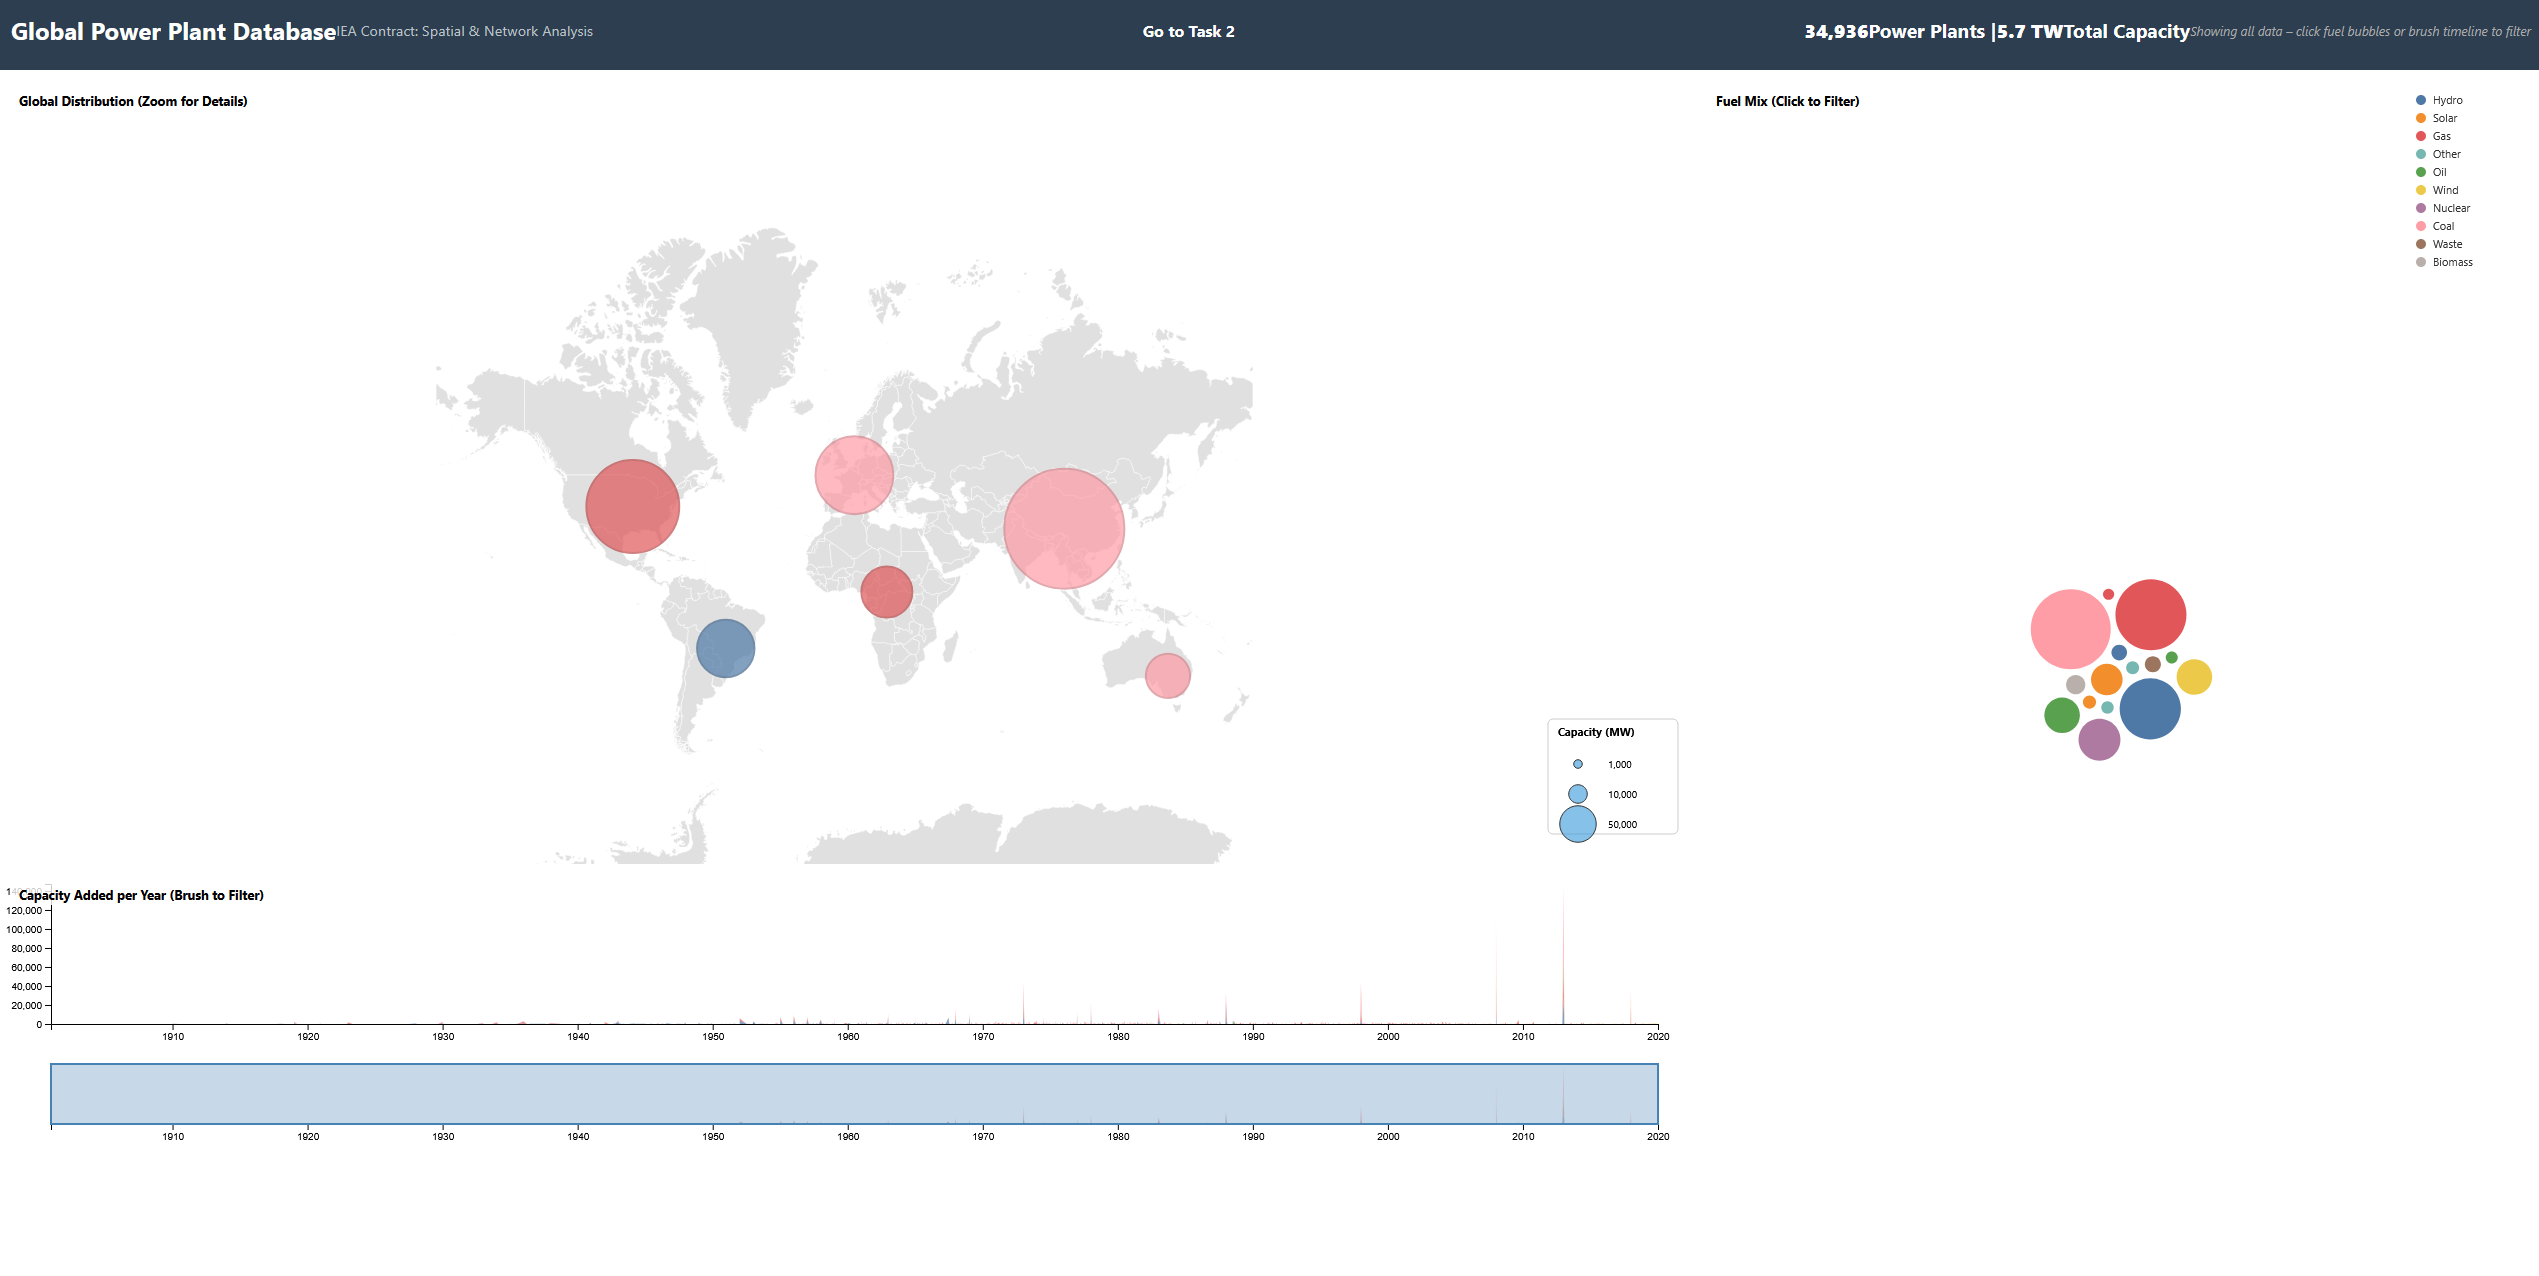
\includegraphics[width=\textwidth]{images/task1.png}
    \caption{Task 1 Dashboard: Power Plant Distribution with Map, Force Layout, and Timeline}
    \label{fig:task1}
\end{figure}

\subsection{Requirement 1.1: Zoomable Aggregate Map}
\textbf{Challenge:} Rendering 35,000 points crashes the browser.\\
\textbf{Solution:} Implemented \textbf{4-level semantic zooming}:
\begin{itemize}[noitemsep]
    \item \textbf{Level 1 (zoom 1.0--2.0):} Regional aggregates (6 continents)
    \item \textbf{Level 2 (zoom 2.0--4.0):} Country-level aggregates with centroid positioning
    \item \textbf{Level 3 (zoom 4.0--6.0):} Grid-based spatial clusters (5° cells)
    \item \textbf{Level 4 (zoom 6.0+):} Individual power plants with viewport culling
\end{itemize}
\textbf{Why:} Progressive disclosure prevents performance issues while maintaining data fidelity at high zoom.

\textbf{Key Implementation:}
\begin{itemize}[noitemsep]
    \item Projection: \texttt{d3.geoMercator()} -- familiar, good continental shapes
    \item Zoom: \texttt{d3.zoom()} with scale extent [1, 12]
    \item Smooth opacity transitions between levels using \texttt{d3.transition()}
    \item Viewport culling limits rendered points to visible bounds + 5000 max
\end{itemize}

\subsection{Requirement 1.2: Force-Directed Fuel Clustering}
\textbf{Implementation:}
\begin{itemize}[noitemsep]
    \item Nodes represent fuel types (Solar, Coal, Nuclear, etc.)
    \item Node radius scaled by total capacity via \texttt{d3.scaleSqrt()}
    \item Forces: \texttt{forceCenter}, \texttt{forceManyBody}, \texttt{forceCollide}, \texttt{forceX/Y}
\end{itemize}
\textbf{Interaction:} Clicking a fuel node filters the entire dashboard. Nodes return to cluster after drag (\texttt{fx/fy = null} on drag end).

\textbf{Why forceCollide:} Prevents node overlap using \texttt{radius + 3px} padding with 3 iterations for stability.

\subsection{Requirement 1.3: Brushable Timeline}
\textbf{Design:} Focus+Context pattern with:
\begin{itemize}[noitemsep]
    \item \textbf{Focus (top):} Detailed stacked area chart responding to brush
    \item \textbf{Context (bottom):} Minimap with \texttt{d3.brushX()} for range selection
\end{itemize}
\textbf{Linked View:} Brush selection updates \texttt{state.filterRange}, triggering map and force layout re-render via \texttt{d3.dispatch("stateChanged")}.

\textbf{Data Handling:} Plants without commissioning years are \textbf{included} when filtering by year range to preserve complete dataset ($\sim$17,000 plants lack year data).

%==============================================================================
\section{Task 2: Temporal \& Hierarchical Simulation (UNDP Gapminder)}
%==============================================================================

\subsection{Overview}
An animated visualization correlating GDP and Life Expectancy from 1800--2023:
\begin{enumerate}[noitemsep]
    \item \textbf{Motion Chart} -- Animated scatter plot with smooth transitions
    \item \textbf{Synchronized Choropleth Map} -- Real-time color updates
    \item \textbf{Interactive Controls} -- D3-drag slider + Sunburst drill-down
\end{enumerate}

\begin{figure}[H]
    \centering
    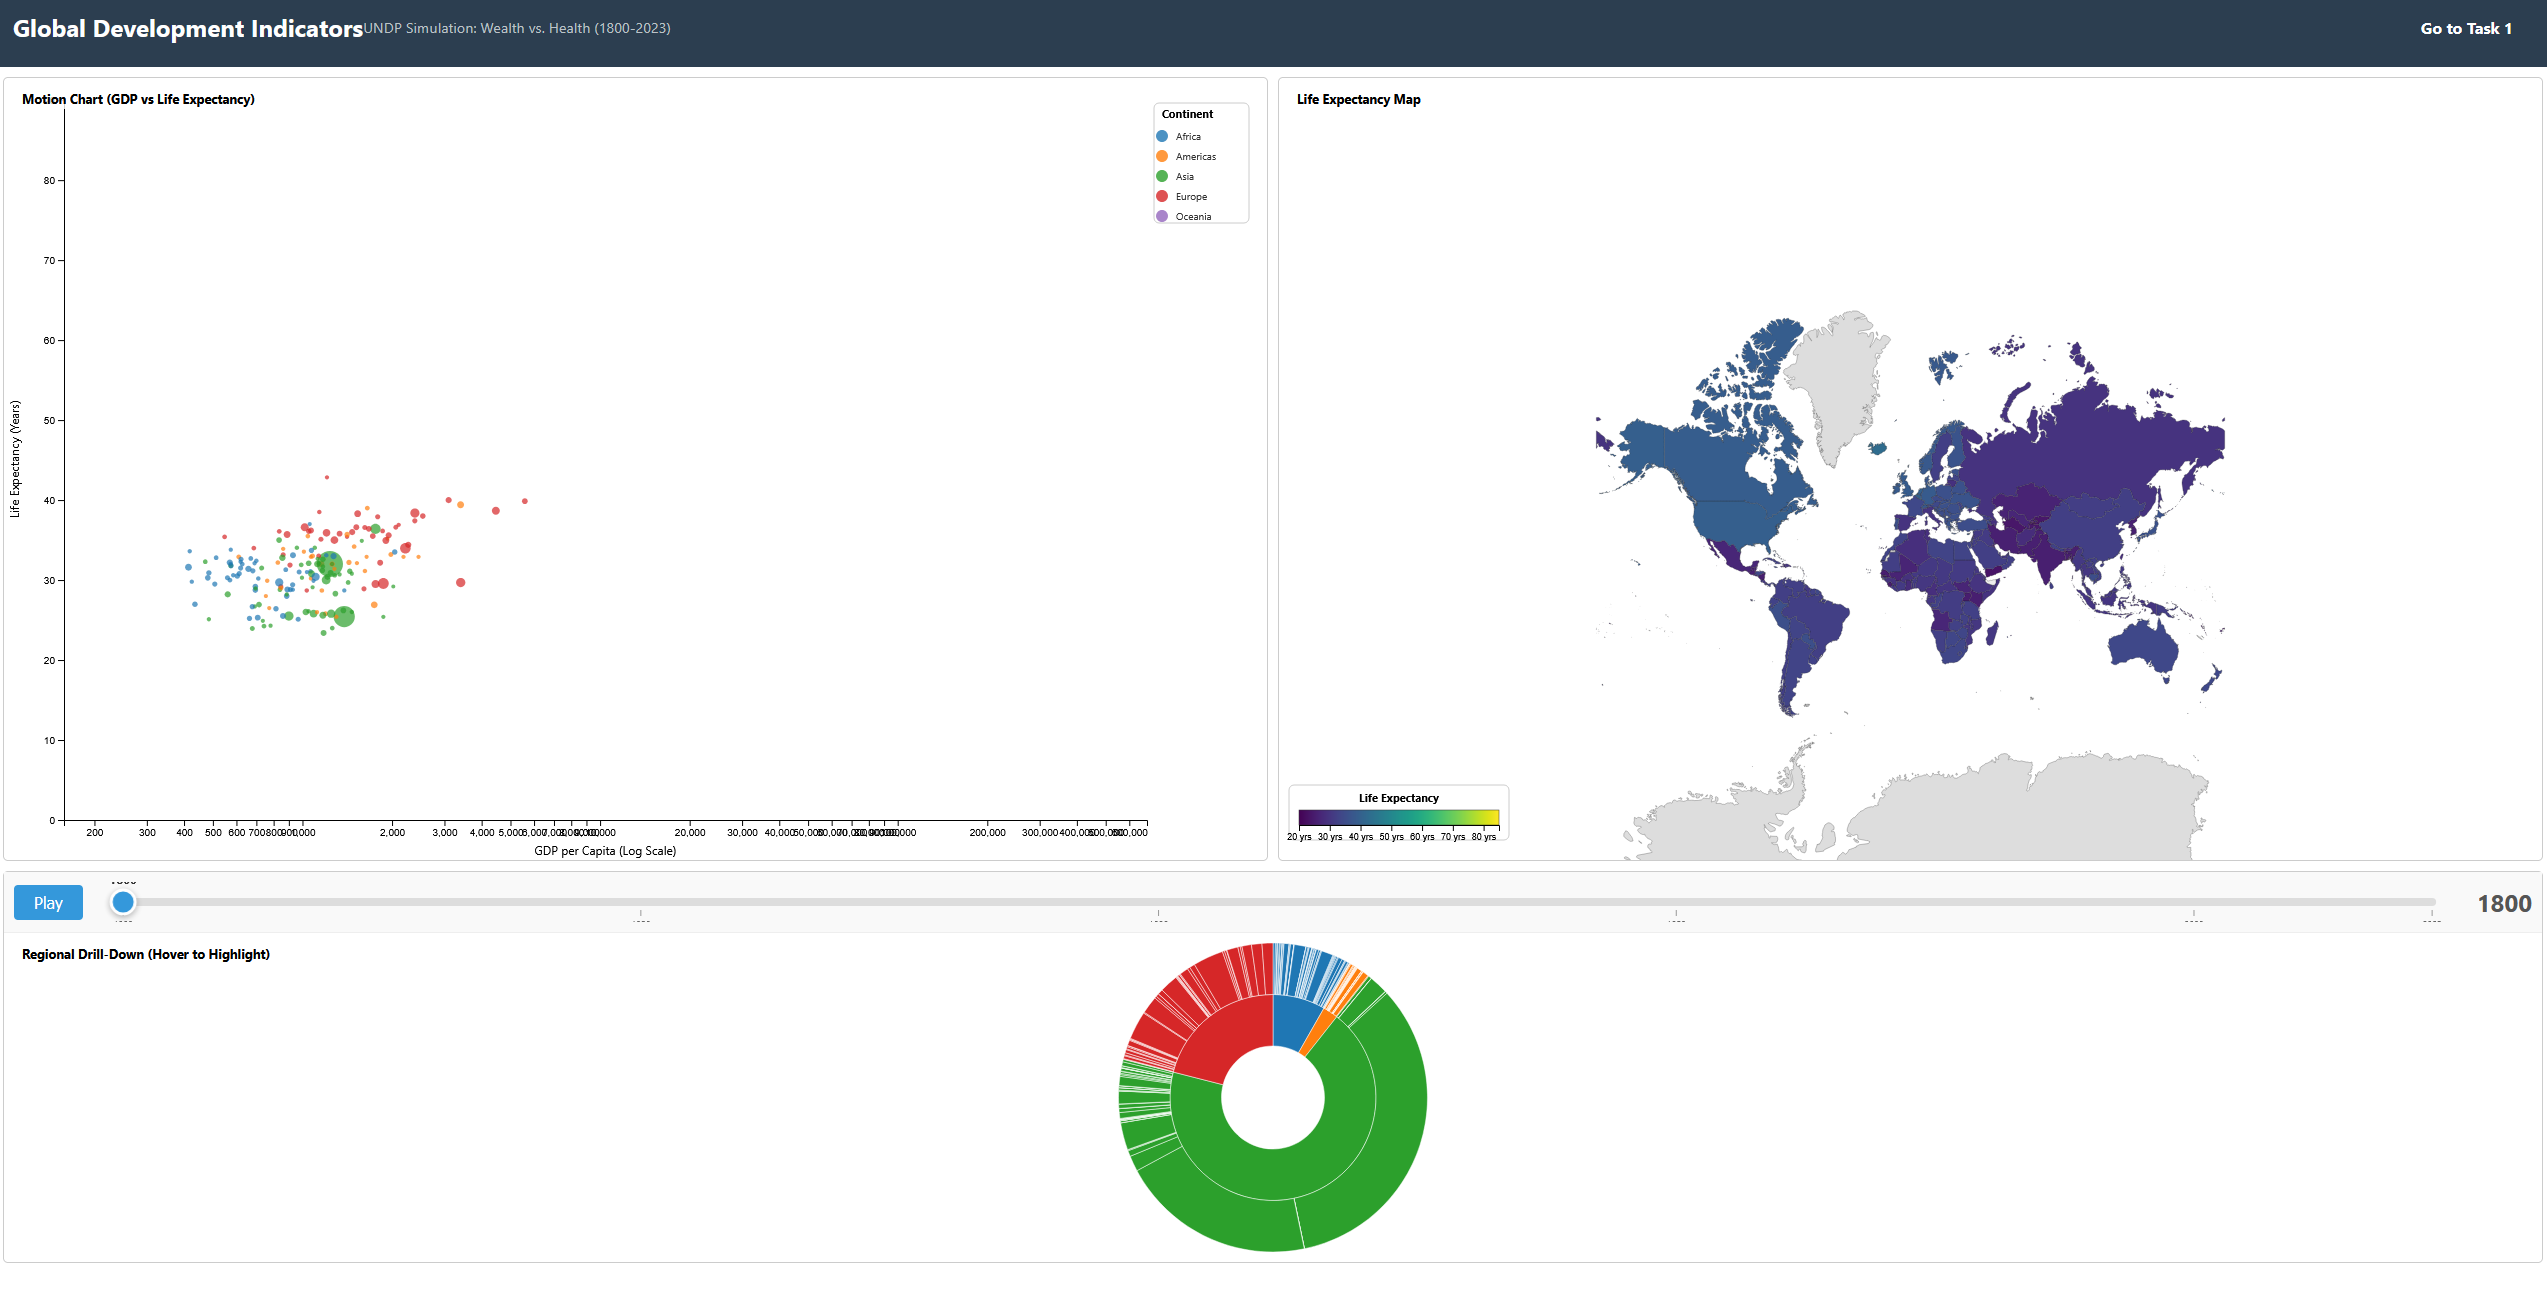
\includegraphics[width=\textwidth]{images/task2.png}
    \caption{Task 2 Dashboard: Motion Chart, Choropleth Map, Slider, and Sunburst Drill-Down}
    \label{fig:task2}
\end{figure}

\subsection{Requirement 2.1: Motion Chart}
\textbf{Scales (as required):}
\begin{itemize}[noitemsep]
    \item X-axis: \texttt{d3.scaleLog()} for GDP per capita
    \item Y-axis: \texttt{d3.scaleLinear()} for Life Expectancy
    \item Radius: \texttt{d3.scaleSqrt()} for Population
    \item Color: \texttt{d3.scaleOrdinal(schemeCategory10)} by continent
\end{itemize}
\textbf{Animation:} Play/Pause via \texttt{d3.interval()} at 200ms per year. Bubbles transition smoothly using \texttt{.transition().duration(200).ease(d3.easeLinear)}.

\textbf{Why Log Scale for GDP:} Income distribution is heavily skewed; log scale reveals patterns in lower-income countries that would be invisible on linear scale.

\subsection{Requirement 2.2: Synchronized Choropleth Map}
\textbf{Implementation:}
\begin{itemize}[noitemsep]
    \item Color scale: \texttt{d3.scaleSequential(interpolateViridis)} domain [20, 85] years
    \item ISO mapping: Numeric TopoJSON IDs → lowercase alpha-3 codes → Gapminder data
    \item Strict synchronization: Map colors update on every year change via \texttt{state2.countryMap}
\end{itemize}
\textbf{Why Viridis:} Perceptually uniform, colorblind-friendly, meaningful progression from dark (low life expectancy) to bright (high).

\subsection{Requirement 2.3: Interactive Controls}
\subsubsection{D3-Drag Year Slider}
\textbf{Critical:} Pure D3 implementation using \texttt{d3.drag()}:
\begin{itemize}[noitemsep]
    \item Track with gradient fill showing progress
    \item Draggable handle with visual feedback (size change, cursor)
    \item Click-to-jump on track
    \item Smooth snap-to-year on drag end
\end{itemize}
\textbf{Why:} Assignment requirement; demonstrates mastery of d3-drag API.

\subsubsection{Sunburst Drill-Down}
\textbf{Hierarchy:} World → Continent → Country using \texttt{d3.hierarchy()} and \texttt{d3.partition()}.\\
\textbf{Interaction:} Hovering dispatches \texttt{hoverContinent} event with both continent and country code:
\begin{itemize}[noitemsep]
    \item \textbf{Continent hover:} Dims all bubbles/countries not in that continent
    \item \textbf{Country hover:} Highlights only that specific country in both views
\end{itemize}

%==============================================================================
\section{Architecture \& Design Decisions}
%==============================================================================

\subsection{Code Modularity}
Files organized by responsibility:
\begin{itemize}[noitemsep]
    \item \texttt{state.js / task2\_main.js} -- Centralized state management
    \item \texttt{utils.js} -- Data loading, filtering, aggregation
    \item \texttt{map.js / choropleth\_map.js} -- Geographic visualizations
    \item \texttt{force.js / motion\_chart.js} -- Non-geographic visualizations
    \item \texttt{timeline.js / controls.js} -- Interactive components
\end{itemize}

\subsection{Event-Driven Communication}
Both dashboards use \texttt{d3.dispatch()} for loose coupling:
\begin{itemize}[noitemsep]
    \item Task 1: \texttt{dataLoaded}, \texttt{stateChanged}, \texttt{zoomChanged}
    \item Task 2: \texttt{yearChanged}, \texttt{playToggled}, \texttt{hoverContinent}, \texttt{dataLoaded}
\end{itemize}
\textbf{Why:} Components don't directly reference each other; changes propagate through events.

\subsection{Performance Optimizations}
\begin{enumerate}[noitemsep]
    \item \textbf{Pre-computed aggregates:} All 4 zoom levels calculated on data load
    \item \textbf{Viewport culling:} Only render visible points at high zoom
    \item \textbf{Data keys:} \texttt{.data(data, d => d.id)} for stable DOM updates
    \item \textbf{Scale clamping:} Prevent rendering outside bounds
\end{enumerate}

%==============================================================================
\section{Challenges \& Solutions}
%==============================================================================

\begin{table}[H]
\centering
\begin{tabular}{@{}p{5cm}p{9cm}@{}}
\toprule
\textbf{Challenge} & \textbf{Solution} \\
\midrule
35,000 points crash browser & 4-level semantic zoom with progressive aggregation \\
ISO code mismatch (TopoJSON vs Gapminder) & Built numeric → alpha-3 mapping from ISO-3166 JSON \\
Bubbles flicker during animation & Proper enter/update/exit pattern with key function \\
Plants missing year data excluded & Modified filter: include NaN years with valid range \\
Sunburst hover only filtered scatter & Added \texttt{choroplethMap.highlight()} method \\
Country-level drill-down non-functional & Extended hover event to pass \texttt{countryCode} \\
\bottomrule
\end{tabular}
\caption{Implementation Challenges and Solutions}
\end{table}

%==============================================================================
\section{Conclusion}
%==============================================================================
Both dashboards successfully implement all requirements using pure D3.js. Key achievements:
\begin{itemize}[noitemsep]
    \item Semantic zooming handles 35,000+ points without performance issues
    \item Force simulation with proper collision detection and re-clustering
    \item Smooth animations using d3-transition and d3-interval
    \item Full view synchronization via event-driven architecture
    \item Custom d3-drag slider as required (not HTML input)
    \item Two-level drill-down filtering (continent and country)
\end{itemize}

\end{document}
